\documentclass{ltjsarticle}
\usepackage[english]{babel}
\usepackage{luatexja}
\usepackage{amsmath,amssymb}
\usepackage{amsthm}
\usepackage{physics} 
\usepackage[dvipdfmx]{graphicx}
\usepackage[dvipdfmx]{color}
\usepackage{booktabs}
\usepackage{siunitx}
\usepackage{comment}
\usepackage{here}
\usepackage{bbm}
\newcolumntype{d}{S[
    input-open-uncertainty=,
    input-close-uncertainty=,
    parse-numbers = false,
    table-align-text-pre=false,
    table-align-text-post=false
 ]}


\usepackage{titlesec}
\titleformat*{\section}{\large\rmfamily}
\titleformat*{\subsection}{\rmfamily}
\titleformat*{\subsubsection}{\rmfamily}

\usepackage{tcolorbox}
\usepackage[legacycolonsymbols]{mathtools}
\usepackage{xcolor}

%python
\usepackage{listings}
\usepackage{xcolor}
\definecolor{codegreen}{rgb}{0,0.6,0}
\definecolor{codegray}{rgb}{0.5,0.5,0.5}
\definecolor{codepurple}{rgb}{0.58,0,0.82}
\definecolor{codered}{rgb}{0.6,0,0}
\definecolor{backcolour}{rgb}{0.95,0.95,0.92}



\newcommand{\s}{\sigma}
\newcommand{\ve}{\varepsilon}
\newcommand{\e}{\epsilon}

\title{Macroeconomics $\mathrm{II}$ Homework 2}
\date{\today}
\author{Graduate School of Economics, The University of Tokyo\\[4mm]29--246029 Rin NITTA\\ 29-246033 Rei HANARI \\ 29--246004 Kosuke IGARASHI
}
\begin{document}
\maketitle



\section{} %1
\subsection*{(a)}
Social planner's problem can be written as below.
\begin{align*}
    &w(k_0) = \max_{\{c_t, k_{t+1}\}_{t=0}^\infty} \sum_{t=0}^\infty \beta^t \log c_t \\
    &\text{s.t.} F(k_t) \= k_t^\alpha\\
    &c_t \geq 0, k_{t+1} \geq 0\\
    &k_0 = 0 given
\end{align*}
Define 
\begin{align*}
    f(k) \equiv F(k) + (1-\delta)k = k^\alpha + (1-\delta)k
\end{align*}
$f$ gives total output and un-depreciated capital that remains.\\
The resource constraint is $c_t + k_{t+1} = k_t^\alpha + (1 - \delta)k_t$.\\
From $c_t \geq 0$ and $k_{t+1} \geq 0$, $0 \leq k_{t+1} \leq k_t^\alpha + (1 - \delta)k_t$ holds.\\
Then, $c_t = k_t^\alpha + (1 - \delta)k_t - k_{t+1}$.\\
Now, the social planner's problem is
\begin{align*}
    w(k_0) \= max_{\{k_{t+1}\}_{t=0}^\infty ,k_0 given} \sum_{t=0}^\infty \beta^t \log (k_t^\alpha + (1 - \delta)k_t - k_{t+1})\\
    \= max_{k_1} \{ \log (k_0^\alpha + (1 - \delta)k_0 - k_1) + \beta [\max_{\{k_{t+1}\}_{t = 1}^\infty ,k_1 given] \sum_{t=1}^\infty \log(k_t^\alpha + (1 - \delta)k_t - k_{t+1})\}\\
    \text{with} 0\leq k_{t+1} \leq k_t^\alpha + (1 - \delta)k_t \text{ for all } t
\end{align*}
From this,
\begin{align*}
    w(k_0) = \max_{0 \leq k_1 \leq k_0^\alpha + (1 - \delta)k_0 , k_0 given} \{ \log (k_0^\alpha + (1 - \delta)k_0 - k_1) + \beta w(k_1)\}
\end{align*}
We introduce value function $v(.)$ for the recursive problem.\\
Therefore, the recursive problem is
\begin{align*}
    v(k) = \max_{0 \leq k' \leq k^\alpha + (1 - \delta)k} \{ \log (k^\alpha + (1 - \delta)k - k') + \beta v(k')\}
\end{align*}

\subsection*{(b)}
The value function and the policy function are shown in the following figures.
\begin{figure}[H]
    \centering
    \begin{minipage}[b]{\textwidth}
        \centering
        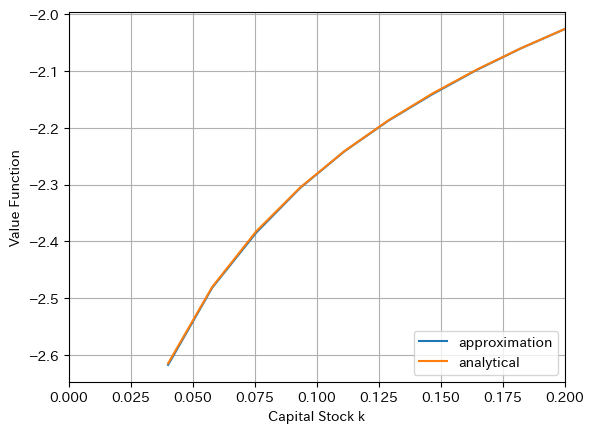
\includegraphics[width=0.3\textwidth]{Q1B_VF.png}
        \caption{Value Function}
        \label{fig:value_function}
    \end{minipage}
    \begin{minipage}[b]{\textwidth}
        \centering
        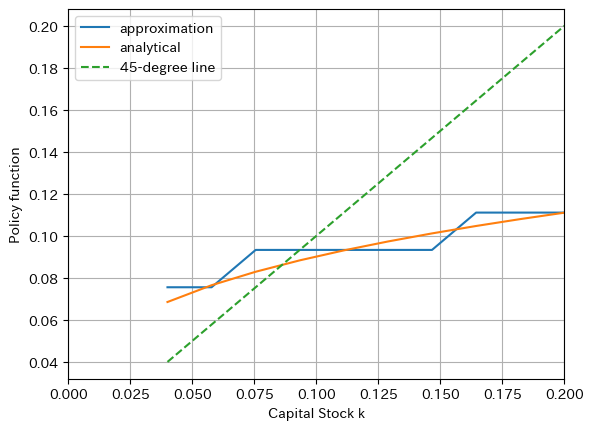
\includegraphics[width=0.3\textwidth]{Q1B_PF.png}
        \caption{Policy Function}
        \label{fig:policy_function}
    \end{minipage}
    \label{fig:value_and_policy_functions}
\end{figure}

The Python code is as follows:
\begin{lstlisting}[language=python,
    backgroundcolor=\color{backcolour},
    commentstyle=\color{codegreen},
    morekeywords={as},
    classoffset=0,
    keywordstyle=\color{codepurple},
    deletekeywords={list,in,float},
    classoffset=1,
    morekeywords={list},
    keywordstyle=\color{blue!60!green},
    classoffset=2,
    morekeywords={in},
    keywordstyle=\color{blue},
    classoffset=3,
    morekeywords={float},
    keywordstyle=\color{blue!40!green},
    numberstyle=\tiny\color{black},
    stringstyle=\color{codered},
    basicstyle=\ttfamily\footnotesize,
    breaklines=true,
    emph={len,range,print},
    emphstyle=\color{yellow!40!black}
    ]
import numpy as np
import matplotlib.pyplot as plt

class Model():
    def __init__(self,
        beta = 0.6,
        gamma = 1.0,
        alpha = 0.3,
        delta = 1.0,
        nk = 10,   
        kmax = 0.2,  
        kmin = 0.04, 
        maxit = 1000,
        tol = 1e-4,  
        ): 
        
        self.beta, self.gamma, self.alpha = beta, gamma, alpha 
        self.delta, self.nk = delta, nk 
        self.kmax, self.kmin = kmax, kmin 
        self.maxit, self.tol = maxit, tol
        self.kgrid = np.linspace(kmin,kmax,nk) 


it = 1
dif1 = 1.0 
dif2 = 1.0 

m = Model()
vfcn = np.ones(m.nk)
pfcn = np.ones_like(vfcn)
Tvfcn = np.zeros_like(vfcn)
Tpfcn = np.zeros_like(vfcn)
vkp = np.empty((m.nk,m.nk))
v_conv = [] 
p_conv = [] 
util = np.ones((m.nk, m.nk))

def utility(c):
    if c > 0:
        return np.log(c)
    else:
        return -1e10 

for i in range(m.nk): 
    for j in range(m.nk): 
        wealth = m.kgrid[i] ** m.alpha + (1.0 - m.delta) * m.kgrid[i]
        cons = wealth - m.kgrid[j]
        util[i, j] = utility(cons) 

while (it<m.maxit) & (dif1>m.tol):

    for i in range(m.nk):
        
        vkp[i,:] = util[i,:] + m.beta*vfcn
        
        ploc = np.argmax(vkp[i,:])
        Tvfcn[i] = vkp[i,ploc]
        Tpfcn[i] = m.kgrid[ploc]
    
    dif1 = np.max(np.abs((Tvfcn-vfcn)/vfcn))
    dif2 = np.max(np.abs((Tpfcn-pfcn)/pfcn)) 
    
    vfcn = np.copy(Tvfcn)
    pfcn = np.copy(Tpfcn)

    print(f"iteration index: {it}, iteration diff of value: {dif1:.7f}")

    v_conv.append(dif1)
    p_conv.append(dif2)

    it += 1

print("-+- PARAMETER VALUES -+-")
print(f"beta={m.beta}, gamma={m.gamma}, alpha={m.alpha}, delta={m.delta}")
print(f"kmin={m.kmin}, kmax={m.kmax}, grid={m.nk}")

AA = (1-m.beta)**(-1) * (np.log(1-m.alpha*m.beta) + ((m.alpha*m.beta)/(1-m.alpha*m.beta))*np.log(m.alpha*m.beta))
BB = m.alpha/(1-m.alpha*m.beta)
v_true = AA + BB*np.log(m.kgrid)
p_true = m.beta * m.alpha * (m.kgrid ** m.alpha)

fig, ax = plt.subplots()
ax.plot(m.kgrid,vfcn,label="approximation")
ax.plot(m.kgrid,v_true,label="analytical")
ax.set(title="",xlabel=r"Capital Stock k", ylabel=r"Value Function",xlim=(0,m.kmax))
ax.legend(loc="lower right")
ax.grid()
plt.show()

fig, ax = plt.subplots()
ax.plot(m.kgrid, pfcn, label="approximation")
ax.plot(m.kgrid, p_true, label="analytical")
ax.plot(m.kgrid, m.kgrid, ls="--", label="45-degree line")
ax.set(title="",xlabel=r"Capital Stock k", ylabel=r"Policy function",xlim=(0,m.kmax))
ax.legend(loc="upper left")
ax.grid()
plt.show()
\end{lstlisting}



\subsection*{(c)}

The value function and the policy function are shown in the following figures.
\begin{figure}[H]
    \centering
    \begin{minipage}[b]{\textwidth}
        \centering
        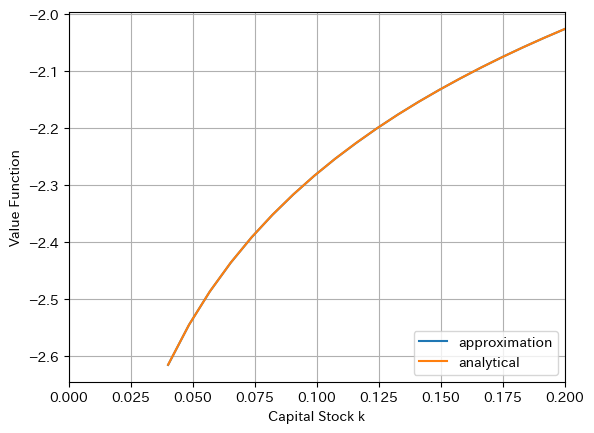
\includegraphics[width=0.3\textwidth]{Q1C_VF.png}
        \caption{Value Function}
        \label{fig:value_function}
    \end{minipage}
    \begin{minipage}[b]{\textwidth}
        \centering
        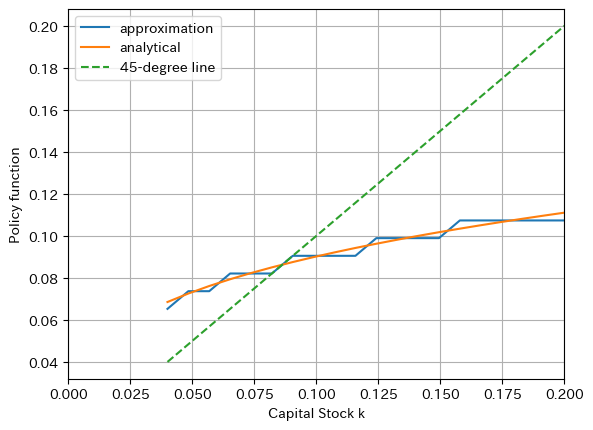
\includegraphics[width=0.3\textwidth]{Q1C_PF.png}
        \caption{Policy Function}
        \label{fig:policy_function}
    \end{minipage}
    \label{fig:value_and_policy_functions}
\end{figure}

The Python code is as follows:
\begin{lstlisting}[language=python,
    backgroundcolor=\color{backcolour},
    commentstyle=\color{codegreen},
    morekeywords={as},
    classoffset=0,
    keywordstyle=\color{codepurple},
    deletekeywords={list,in,float},
    classoffset=1,
    morekeywords={list},
    keywordstyle=\color{blue!60!green},
    classoffset=2,
    morekeywords={in},
    keywordstyle=\color{blue},
    classoffset=3,
    morekeywords={float},
    keywordstyle=\color{blue!40!green},
    numberstyle=\tiny\color{black},
    stringstyle=\color{codered},
    basicstyle=\ttfamily\footnotesize,
    breaklines=true,
    emph={len,range,print},
    emphstyle=\color{yellow!40!black}
    ]
import numpy as np
import matplotlib.pyplot as plt

class Model():
    def __init__(self,
        beta = 0.6,  
        gamma = 1.0,
        alpha = 0.3,  
        delta = 1.0,  
        nk = 20,   
        kmax = 0.2, 
        kmin = 0.04, 
        maxit = 1000,
        tol = 1e-4,  
        ): 
        
        self.beta, self.gamma, self.alpha = beta, gamma, alpha 
        self.delta, self.nk = delta, nk 
        self.kmax, self.kmin = kmax, kmin 
        self.maxit, self.tol = maxit, tol
        self.kgrid = np.linspace(kmin,kmax,nk) 

it = 1 
dif1 = 1.0 #価値関数の繰り返し誤差
dif2 = 1.0 #政策関数の繰り返し誤差

m = Model()
vfcn = np.ones(m.nk)
pfcn = np.ones_like(vfcn)
Tvfcn = np.zeros_like(vfcn)
Tpfcn = np.zeros_like(vfcn)
vkp = np.empty((m.nk,m.nk))
v_conv = [] 
p_conv = [] 

util = np.ones((m.nk, m.nk))

def utility(c):
    if c > 0:
        return np.log(c)
    else:
        return -1e10 

for i in range(m.nk):
    for j in range(m.nk): 
        wealth = m.kgrid[i] ** m.alpha + (1.0 - m.delta) * m.kgrid[i]
        cons = wealth - m.kgrid[j]
        util[i, j] = utility(cons) 

while (it<m.maxit) & (dif1>m.tol):

    for i in range(m.nk):
        
        vkp[i,:] = util[i,:] + m.beta*vfcn
        
        ploc = np.argmax(vkp[i,:])
        Tvfcn[i] = vkp[i,ploc]
        Tpfcn[i] = m.kgrid[ploc]
    
    dif1 = np.max(np.abs((Tvfcn-vfcn)/vfcn))
    dif2 = np.max(np.abs((Tpfcn-pfcn)/pfcn)) 
    
    vfcn = np.copy(Tvfcn)
    pfcn = np.copy(Tpfcn)

    print(f"iteration index: {it}, iteration diff of value: {dif1:.7f}")

    v_conv.append(dif1)
    p_conv.append(dif2)

    it += 1

print("-+- PARAMETER VALUES -+-")
print(f"beta={m.beta}, gamma={m.gamma}, alpha={m.alpha}, delta={m.delta}")
print(f"kmin={m.kmin}, kmax={m.kmax}, grid={m.nk}")

AA = (1-m.beta)**(-1) * (np.log(1-m.alpha*m.beta) + ((m.alpha*m.beta)/(1-m.alpha*m.beta))*np.log(m.alpha*m.beta))
BB = m.alpha/(1-m.alpha*m.beta)
v_true = AA + BB*np.log(m.kgrid)
p_true = m.beta * m.alpha * (m.kgrid ** m.alpha)


fig, ax = plt.subplots()
ax.plot(m.kgrid,vfcn,label="approximation")
ax.plot(m.kgrid,v_true,label="analytical")
ax.set(title="",xlabel=r"Capital Stock k", ylabel=r"Value Function",xlim=(0,m.kmax))
ax.legend(loc="lower right")
ax.grid()
plt.show()

fig, ax = plt.subplots()
ax.plot(m.kgrid, pfcn, label="approximation")
ax.plot(m.kgrid, p_true, label="analytical")
ax.plot(m.kgrid, m.kgrid, ls="--", label="45-degree line")
ax.set(title="",xlabel=r"Capital Stock k", ylabel=r"Policy function",xlim=(0,m.kmax))
ax.legend(loc="upper left")
ax.grid()
plt.show()
\end{lstlisting}


\section{} %2 Nitta

\subsection*{(a)}

At the optimal consumption, the budget constraint holds with equality:
\begin{gather*}
    c_t = A k_t^\alpha - k_{t+1}
\end{gather*}

Define 
\begin{gather*}
    w(k_0) = \max_{\{k_{t+1}\}_{t=0}^\infty} \sum_{t=0}^\infty \beta^t \log c_t
\end{gather*}
Then, this is equivalent to
\begin{align*}
    w(k_0) 
    &= \max_{\{k_{t+1}\}_{t=0}^\infty ; k_0 \: \text{given}} \sum_{t=0}^\infty \beta^t \log c_t \\
    &= \max_{k_1; k_0 \: \text{given}} \log c_0 + \beta \left[\max_{\{k_{t+1}\}_{t=1}^\infty ; k_1 \: \text{given}} \sum_{t=1}^\infty \beta^{t-1} \log c_t \right] \\
    &= \max_{k_1; k_0 \: \text{given}} \log (A k_0^\alpha - k_1) + \beta w(k_1)
\end{align*}
with conditions $0 \leq k_1 \leq A k_0^\alpha$ for all $t = 0, \cdots, \infty$. This is the recursive problem of the social planner.

\subsection*{(b)}
\subsubsection*{(i): Guess and Verify}
Guess $V(k) = X + Y \log A k^\alpha$ where $X$ and $Y$ are coefficients to be determined.
Then, the Bellman equation is
\begin{gather*}
    V(k) = \max_{0 \leq k' \leq  A k^\alpha; k \: \text{given}} \log (A k^\alpha - k') + \beta (X + Y \log A k'^\alpha)
\end{gather*}
The first-order condition is
\begin{gather*}
    \frac{\partial V(k)}{\partial k'} = - \frac{1}{A k^\alpha - k'} + \alpha \beta Y \frac{1}{k'} = 0\\
    \therefore \quad k' = \frac{\alpha \beta Y}{1 + \alpha \beta Y} A k^\alpha
\end{gather*}

Evaluating the objecting function (RHS) at the optimal $k'$, we have
\begin{align*}
    (RHS)
    &= \log \left( A k^\alpha - \frac{\alpha \beta Y}{1 + \alpha \beta Y} A k^\alpha \right) + \beta (X + Y \log A \left( \frac{\alpha \beta Y}{1 + \alpha \beta Y} A k^\alpha \right)^\alpha) \\
    &= \beta X + \log \left( \frac{1}{1+\alpha\beta Y}\right) + \alpha\beta Y \log \left( \frac{\alpha \beta Y}{1+\alpha \beta Y}\right) + \beta Y \log A + (1+\alpha\beta Y) \log(A k^\alpha)
\end{align*}
Solving this, we have
\begin{align*}
    X &= \frac{1}{1-\beta} \left[ \log \left( 1-\alpha\beta \right) +  \frac{\alpha \beta}{1 - \alpha \beta} \log \left( \alpha \beta \right)  \right] \\
    Y &= \frac{1}{1-\alpha\beta} 
\end{align*}
Thus, the value function is represented as the form of $V(k) = C + \frac{1}{1-\alpha\beta}\log A k^\alpha$. 

\subsubsection*{(ii): Value Function Iteration}

We set the value of parameters as follows:
\begin{gather*}
    \beta = 0.6, \quad \alpha = 0.3, \quad \delta = 1.0, \quad A = 1.0, \\ nk = 100, \quad k_{\max} = 0.2, \quad k_{\min} = 0.04, \quad \text{maxit} = 10000, \quad \text{tol} = 1e-5
\end{gather*}

The value function and the policy function are shown in the following figures. We used the result of Guess and Verify as the true value function and policy function.
\begin{figure}[H]
    \centering
    \begin{minipage}[b]{\textwidth}
        \centering
        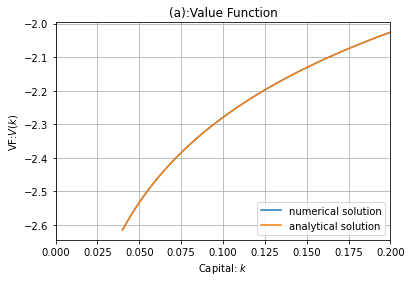
\includegraphics[width=0.3\textwidth]{Q2_VF.png}
        \caption{Value Function}
        \label{fig:value_function}
    \end{minipage}
    \begin{minipage}[b]{\textwidth}
        \centering
        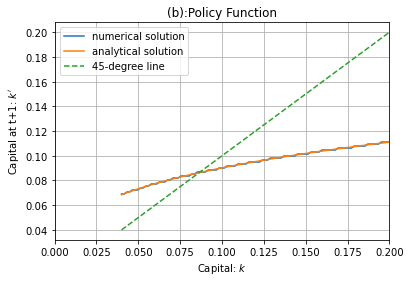
\includegraphics[width=0.3\textwidth]{Q2_PF.png}
        \caption{Policy Function}
        \label{fig:policy_function}
    \end{minipage}
    \label{fig:value_and_policy_functions}
\end{figure}

The Python code is as follows:
\begin{lstlisting}[language=python,
    backgroundcolor=\color{backcolour},
    commentstyle=\color{codegreen},
    morekeywords={as},
    classoffset=0,
    keywordstyle=\color{codepurple},
    deletekeywords={list,in,float},
    classoffset=1,
    morekeywords={list},
    keywordstyle=\color{blue!60!green},
    classoffset=2,
    morekeywords={in},
    keywordstyle=\color{blue},
    classoffset=3,
    morekeywords={float},
    keywordstyle=\color{blue!40!green},
    numberstyle=\tiny\color{black},
    stringstyle=\color{codered},
    basicstyle=\ttfamily\footnotesize,
    breaklines=true,
    emph={len,range,print},
    emphstyle=\color{yellow!40!black}
    ]
class Model():
    def __init__(self,
        beta = 0.6,
        alpha = 0.3,  
        delta = 1.0, 
        A = 1.0,     
        nk = 100,   
        kmax = 0.2,  
        kmin = 0.04, 
        maxit = 10000, 
        tol = 1e-5,
        ): 
        
        self.beta, self.alpha = beta, alpha 
        self.delta, self.nk = delta, nk 
        self.A = A
        self.kmax, self.kmin = kmax, kmin 
        self.maxit, self.tol = maxit, tol
        self.kgrid = np.linspace(kmin,kmax,nk)


it = 1 
dif1 = 1.0 
dif2 = 1.0 

m = Model()
vfcn = np.ones(m.nk)
pfcn = np.ones_like(vfcn)
Tvfcn = np.zeros_like(vfcn)
Tpfcn = np.zeros_like(vfcn)
vkp = np.empty((m.nk,m.nk))
v_conv = [] 
p_conv = [] 
util = np.ones((m.nk,m.nk))

for i in range(m.nk): #k
    for j in range(m.nk): #k'
        
        wealth = m.A * m.kgrid[i] ** m.alpha + (1.0-m.delta)*m.kgrid[i] #A k^\alpha
        cons = wealth - m.kgrid[j] # A k^\alpha - k'
        util[i,j] = np.log(cons) # log(A k^\alpha - k')

while (it<m.maxit) & (dif1>m.tol):

    for i in range(m.nk):
        
        vkp[i,:] = util[i,:] + m.beta*vfcn
        
        ploc = np.argmax(vkp[i,:])
        Tvfcn[i] = vkp[i,ploc]
        Tpfcn[i] = m.kgrid[ploc]
    
    dif1 = np.max(np.abs((Tvfcn-vfcn)/vfcn))
    dif2 = np.max(np.abs((Tpfcn-pfcn)/pfcn)) 
    
    vfcn = np.copy(Tvfcn)
    pfcn = np.copy(Tpfcn)

    print(f"iteration index: {it}, iteration diff of value: {dif1:.7f}")

    v_conv.append(dif1)
    p_conv.append(dif2)

    it += 1

print("-+- PARAMETER VALUES -+-")
print(f"beta={m.beta} alpha={m.alpha}, delta={m.delta}")
print(f"kmin={m.kmin}, kmax={m.kmax}, grid={m.nk}")

# True value function
AA = (1-m.beta)**(-1) * (np.log(1-m.alpha*m.beta) + ((m.alpha*m.beta)/(1-m.alpha*m.beta))*np.log(m.alpha*m.beta))
BB = m.alpha/(1-m.alpha*m.beta)
v_true = AA + BB*np.log(m.kgrid)
p_true = m.beta * m.alpha * (m.kgrid ** m.alpha)

fig, ax = plt.subplots()
ax.plot(m.kgrid,vfcn,label="numerical solution")
ax.plot(m.kgrid,v_true,label="analytical solution")
ax.set(title="(a):Value Function",xlabel=r"Capital: $k$", ylabel=r"VF:$V(k)$",xlim=(0,m.kmax))
ax.legend(loc="lower right")
ax.grid()
plt.show()

fig, ax = plt.subplots()
ax.plot(m.kgrid, pfcn, label="numerical solution")
ax.plot(m.kgrid, p_true, label="analytical solution")
ax.plot(m.kgrid, m.kgrid, ls="--", label="45-degree line")
ax.set(title="(b):Policy Function",xlabel=r"Capital: $k$", ylabel=r"Capital at t+1: $k'$",xlim=(0,m.kmax))
ax.legend(loc="upper left")
ax.grid()
plt.show()
\end{lstlisting}


\subsubsection*{(iii): Policy Function Iteration}
Using the result in (i), we have the true policy function:
\begin{gather*}
    k' = \frac{\alpha \beta Y}{1 + \alpha \beta Y} A k^\alpha = \alpha \beta A k^\alpha
\end{gather*}
Using this policy function, we can caluculate the value function.
\begin{align*}
    V_{h_j}(k_0) 
    &= \sum_{t=0}^{\infty} \beta^t \log \left(A k_t^\alpha - \beta A k^\alpha \right) \\
    &= \sum_{t=0}^{\infty} \beta^t \log k_t^\alpha + \frac{1}{1-\beta}\log A + \frac{1}{1-\beta}\log (1-\alpha\beta)\\
    &= \frac{\alpha}{1-\alpha\beta}\log k_0 + \frac{1-\beta+ \alpha\beta}{(1-\beta)^2}\log ((1-\alpha\beta)A) 
\end{align*}

Let $D$ be the terms not depending on $k_0$ in the right hand side of $V_{h_j}(k_0)$. Then,
\begin{gather*}
    V_{h_j}(k_0) = \frac{\alpha}{1 - \alpha \beta} \log k_0 + D
\end{gather*}
From now on, find the $k'$ that maximizes
\begin{align*}
    \log(A k^\alpha - k') + \beta V_{h_j}(k')
    &= \log(A k^\alpha - k') + \frac{\alpha \beta}{1 - \alpha \beta} \log k' + \beta D\\
    &= \log \left( (A k^\alpha - k') k'^{\frac{\alpha \beta}{1 - \alpha \beta} }\right)+ \beta D
\end{align*}
The first order condition is
\begin{gather*}
    - k'^{\frac{\alpha \beta}{1 - \alpha \beta}} + \frac{\alpha \beta}{1 - \alpha \beta}(A k^\alpha - k')k'^{\frac{\alpha \beta}{1 - \alpha \beta} -1} = 0\\
    \therefore \quad k' = h_{j+1}(k) =  \alpha \beta A k^\alpha
\end{gather*}
Now, $h_{j+1} (k) = h_{j}(k)= \alpha \beta A k^\alpha$, so the the policy function converges.

Thus, we have
\begin{align*}
    V(k) 
    &= \frac{\alpha}{1 - \alpha \beta} \log k + \frac{1}{1-\alpha\beta} \log A + \text{constant}\\
    &= \frac{1}{1 - \alpha \beta} \log (A k^\alpha) + \text{constant}
\end{align*}


\section{} %3 Nitta

\subsection*{(a)}
The agent's life-time budget constraint is
\begin{gather*}
    \sum_{t=0}^\infty p_t \left(c_t + \frac{b_{t+1}}{1+r_{t+1}} - b_t - e \right)
\end{gather*}

\subsection*{(b)}
Define the Lagrangian as
\begin{gather*}
    \mathcal{L} = \sum_{t=0}^\infty \beta^t \left[ \log c_t + \lambda_t \left( p_t \left(c_t + \frac{b_{t+1}}{1+r_{t+1}} - b_t - e \right) \right) \right] 
\end{gather*}
The first-order conditions are
\begin{align*}
    \frac{\partial \mathcal{L}}{\partial c_t} &= U'(c_t) - \lambda_t p_t = 0 \\
    \frac{\partial \mathcal{L}}{\partial b_t+1} &= - \beta^t \frac{\lambda_t p_t}{1+r_{t+1}} + \beta^{t+1} \lambda_{t+1} p_{t+1} = 0
\end{align*}
Thus, the Euler equation is
\begin{gather*}
    U'(c_t) = \beta U'(c_{t+1})(1+r_{t+1}) \tag{EE}
\end{gather*}
The transversality condition is
\begin{gather*}
    \lim_{t \to \infty} \beta^t (1+r_{t+1}) U'(c_t) b_t = 0 \tag{TVC}
\end{gather*}
with $c_t = b_t - \frac{b_{t+1}}{1 + r_{t+1}} + e$.

\subsection*{(c)}
Suppose (EE) and (TVC) hold. Iterating (EE) backward, we have
\begin{align*}
    U'(c_t) 
    &= \frac{1}{\beta (1+r_{t})} U'(c_{t-1})\\
    &= \frac{1}{\beta (1+r_{t})} \frac{1}{\beta (1+r_{t-1})} U'(c_{t-2})\\
    &= \cdots \\
    &= \frac{1}{\beta^t} U'(c_{0}) \prod_{\tau=1}^{t} \frac{1}{1+r_{\tau}}
\end{align*}
Thus, we have
\begin{gather*}
    \prod_{\tau=1}^{t} \frac{1}{1+r_{\tau}} = \beta^t \frac{U'(c_t)}{U'(c_0)}
\end{gather*}
Substituting this into the left hand side of (NPG), we have
\begin{gather*}
    (LHS) = \frac{1}{U'(c_0)} \lim_{t \to \infty} \beta^t U'(c_t) b_t
\end{gather*}
As for (TVC), it hods that
\begin{gather*}
    |\beta^t (1+r_{t+1}) U'(c_t) b_t| \geq |\beta^t U'(c_t) b_t| \geq 0
\end{gather*}
for all $t$, since $r_{t+1}>0$.
Because $\lim_{t \to \infty} |\beta^t (1+r_{t+1}) U'(c_t) b_t| = 0$ by (TVC), then $\lim_{t \to \infty} |\beta^t U'(c_t) b_t| = 0$ also holds. Therefore, $\lim_{t \to \infty} \beta^t U'(c_t) b_t = 0$. Here, (NPG) condition is met, especially with equality.



\section{} %4
\subsection*{(a)}
\begin{align*}
    v(k,K)= \max_{c,k\geq 0} U(c) + v(k', K')\\
    s.t.\ c+k' &= w(K) + (1+r(K)-\delta -\tau)k + T\\
    K' &= H(K)
\end{align*}

\subsection*{(b)}
RCE is a value function $v:\mathbb{R}^2_{+}\rightarrow \mathbb{R}$ and policy function $C,G:\ \mathbb{R}^2_{+}\rightarrow \mathbb{R}_{+}$ for the representative household, pricing function $w,r:\ \mathbb{R}\rightarrow \mathbb{R}_{+}$ and an aggregate law of motion $H:\ \mathbb{R}_{+}\rightarrow \mathbb{R}_{+}$ such that
\begin{itemize}
    \item[1] Given $w,r,H$, $v$ solves the Bellman equation and $C,G$ are the associated policy function.
    \item[2] Pricing function satisfies firm's FOC.
    \item[3] Consistency for all $K\in \mathbb{R}_{+}$: $H(K) = G(K,K)$
    \item[4] Market clearing: for all $K\in \mathbb{R}_{+}$
    $$C(K,K)+G(K,K) = F(K,1) + (1-\delta)K$$.
\end{itemize}

\subsection*{(c)}
From market clear,
\begin{gather*}
    k_t^d = k_t^s\\
    c_t+k_{t+1}=f(k_t).
\end{gather*}

Thus law of motion for aggregate capital stock is 
\begin{align*}
    K' = H(K)=f(K)-C(K,K).
\end{align*}

\subsection*{(d)}
In the steady state, $K_{t+1}=K_t = K^{*}$. Thus $I=\delta K^{*}$
From market clear
\begin{align*}
    I=\delta K^{*} &= F(K^{*},1) - C(K^{*},K^{*})\\
    K^{*} &=\frac{1}{\delta} \qty{F(K^{*},1) - C(K^{*},K^{*})}
\end{align*}


\subsection*{(e)}
Law of motion for aggregate variables coincide with CE allocation for representative household and firm.

In CE, Firm solves
\begin{align*}
    \max_{\{c_t, k_{t+1}\}^{\infty}_{t=0}} \sum^{\infty}_{t=0} p_t\qty(F(K^d_t,1)-w_t -r_tk_t^d)
\end{align*}

From FOC and assumption of F($\cdot$),
\begin{align*}
    F_K(k_t^d,1)&=r_t\\
    F_N(k_t^d,1)&=w_t\\
    \max_{\{c_t, k_{t+1}\}^{\infty}_{t=0}} \sum^{\infty}_{t=0} p_t\qty(F(K^d_t,1)-w_t -r_tk_t^d)&=0.
\end{align*}

Representative household solves
\begin{align*}
    \max_{\qty{c_t,k_{t+1}}^{\infty}_{t=0}} \sum^{\infty}_{t=0} U(c_t)\\
    s.t.\\
    \sum^{\infty}_{t=0} P_t\qty(c_t + i_t) \leq \sum^{\infty}_{t=0} P_t \qty(w_t+k_t r_t).
    c_t, k_{t+1} \geq 0
    c_t + i_t = k_{t+1} + (1-\delta)k_t
\end{align*}

Note that we do not have to consider the tax because government pay back all taxes.

Define Lagrangian as 
$$\mathcal{L}=\sum^{\infty}_{t=0} U(c_t) + \mu\qty[ \sum^{\infty}_{t=0} P_t \qty(w_t+k_t r_t) - \sum^{\infty}_{t=0} P_t\qty(c_t + i_t)].$$

From FOCs
\begin{align*}
    \beta^t U'(c_t)=\mu P_t\\
    P_{t+1}r_{t+1} -P_t + (1-\delta)P_{t+1}=0.
\end{align*}
Combining, we have Euler equation
\begin{align*}
    U'(c_t)=\beta U'(c_{t+1})(1+r_{t+1}-\delta).
\end{align*}

From $F(K,N)=AK^\alpha L^{1-\alpha}$, and firm's FOC $F_K(K,1)=r_t$

\begin{align*}
    U'(C(K^{*},K^{*}))&=\beta U'(C(K^{*},K^{*}))(1+F_K^{*}(K^{*},1)-\delta)\\
    1&=\beta (1+A\alpha (K^{*})^{\alpha-1}-\delta)\\
    K^{*}&=\qty{\frac{1-\beta(1-\delta)}{\alpha A}}^{\frac{1}{\alpha-1}}
\end{align*}

\section{} %5
The aggregate resource constraint is
\begin{gather*}
    (1+n)^t c_t + K_{t+1} = F(K_t, (1+n)^t (1+g)^t) + (1-\delta)K_t
\end{gather*}
Define growth-adjusted per-capita variables as
\begin{align*}
    \tilde{c}_t &= \frac{c_t}{(1+n)^t} \\
    \tilde{k}_t &= \frac{k_t}{(1+n)^t} = \frac{k_t}{(1+n)^t(1+g)^t} \\
\end{align*}
Divide the aggregate resource constraint by $L_t$, we have
\begin{gather*}
    \tilde{c}_t + (1+n)(1+g) \tilde{k}_{t+1} = f(\tilde{k}_t),\\
    \text{where} \quad f(\tilde{k}_t) = F(\tilde{k}_t, 1) + (1-\delta)\tilde{k}_t.
\end{gather*}
Rewrite the objective function as
\begin{gather*}
    \sum_{t=0}^\infty \beta^t \frac{c_{t}^{1-\sigma}}{1-\sigma} 
    = \sum_{t=0}^\infty \tilde{\beta}^t \frac{\tilde{c}_{t}^{1-\sigma}}{1-\sigma},\\
    \text{where} \quad \tilde{\beta} = \beta (1+n)^{1-\sigma} < 1.
\end{gather*}
Then, the social planner's problem becomes
\begin{gather*}
    \max_{\{\tilde{c}_t, \tilde{k}_{t+1}\}^{\infty}_{t=0}} \sum_{t=0}^\infty \tilde{\beta}^t \frac{\tilde{c}_{t}^{1-\sigma}}{1-\sigma} \\
    \text{s.t.} \quad \tilde{c}_t + (1+n)(1+g) \tilde{k}_{t+1} = f(\tilde{k}_t).
\end{gather*}

The Lagrangian is
\begin{gather*}
    \mathcal{L} = \sum_{t=0}^\infty \tilde{\beta}^t \left[ \frac{\tilde{c}_{t}^{1-\sigma}}{1-\sigma} + \sum_{t=0}^\infty \lambda_t  f(\tilde{k}_t) - \tilde{c}_t - (1+n)(1+g) \tilde{k}_{t+1} \right].
\end{gather*}
The first-order conditions are
\begin{align*}
    \frac{\partial \mathcal{L}}{\partial \tilde{c}_t} &= \tilde{\beta}^t ( \tilde{c}_{t}^{-\sigma} - \lambda_t) = 0, \\
    \frac{\partial \mathcal{L}}{\partial \tilde{k}_{t+1}} &= - \tilde{\beta}^t \lambda_t (1+n)(1+g) +  \tilde{\beta}^{t+1} \lambda_{t+1} \frac{\partial f(\tilde{k}_{t+1})}{\partial \tilde{k}_{t+1}}\\
    &= - \tilde{\beta}^t \lambda_t (1+n)(1+g) +  \tilde{\beta}^{t+1} \lambda_{t+1}[F'(\tilde{k}_{t+1},1)+1-\delta]\\
    &= 0
\end{align*}
From these equations, we can derive the Euler equation as follows:
\begin{gather*}
    \tilde{c}_t^{-\sigma} = \frac{\tilde{\beta}}{(1+n)(1+g)} [F'(\tilde{k}_{t+1},1)+1-\delta] \tilde{c}_{t+1}^{-\sigma} \\
\end{gather*}





\section{} %6
For any $\{k_{t+1} \}^{\infty}_{t=0}$, denote log difference as $\dot{x}_{t+1}= \log(x_{t+1})-\log(x_{t})$.\\
Under BGP, for all $t$,  $\dot{y}_t = \dot{k}_t = 3$
\begin{align*}
    \dot{y}_t &= \alpha \dot{k}_t + (1-\alpha)(\dot{z}_t + \dot{l}_t)\\
    3&= 0.4*0.3 + (1-0.4)(\dot{z}_t + \dot{l}_t)\\
    \dot{z}_t &= 2.
\end{align*}

Thus growth rate of TFP along the balanced growth path is $2\%$.
\end{document}
